\documentclass{article}

\usepackage{booktabs}
\usepackage{graphicx}
\usepackage{caption}
\usepackage{subcaption}

\graphicspath{{../dev/}}

\title{Strategy Analysis: Progressive Entry}
\author{Ivan Anich}

\begin{document}
\maketitle

\section{signal}

up 20\% from the open, \(1<= previous close <= 2\)

\section{Strategy: Add Every 5\%, Exit at 11}

enter short position at 20\% (if occurs between 9:30 and 11), add positions twice as big as the last each time the stock increases another 5\%, only exit at 11.

65 trades between February 26th and May 28th. 

\subsection{Analysis}

high correlation between number of entries and percent return: the more it goes up, the better.

\begin{itemize}
	\item histogram
		
	\begin{figure}
	\center{Histogram of Trades by Number of Entries for Unlimited Adds, Exit at 11 a.m.}
	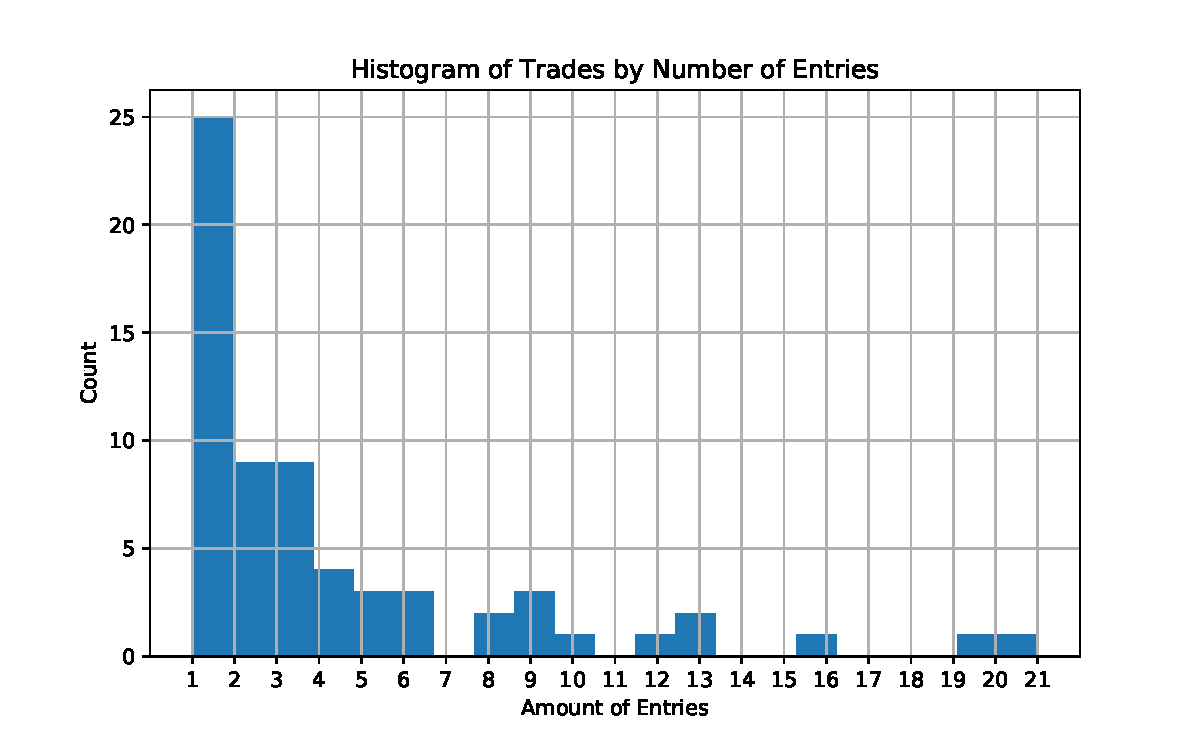
\includegraphics[width=\textwidth]{prog_entry_hist.pdf}
	\caption{This table shows counts of the numbers of trades that had a certain amount of entries. For example, it says that 25 trades had only 1 entry, and that 3 trades had 5 entries (fist entry and 4 adds).}
	\label{hist_strat}
	\end{figure}
	
	\item three tables
	
\begin{table}
\caption{Performance of Default Strategy}
\center{Overall}
\\[2ex]
\begin{tabular}{lcccc}
\hline
         &   0.1    &   0.9    &  median  & average   \\
\midrule
\midrule
constant & -0.0041  & 0.2483   & 0.0924   & 0.1020    \\
         & (0.0140) & (0.0271) & (0.0182) & (0.0123)  \\
N        & 65       & 65       & 65       & 65        \\
Win rate & 0.86     & 0.86     & 0.86     & 0.86      \\
\hline
\end{tabular}

\center{Winners}
\\[2ex]
\begin{tabular}{lcccc}
\hline
         &   0.25   &   0.75   &  median  & average   \\
\midrule
\midrule
constant & 0.0467   & 0.1611   & 0.1130   & 0.1220    \\
         & (0.0163) & (0.0199) & (0.0185) & (0.0123)  \\
N        & 56       & 56       & 56       & 56        \\
Win rate & 0.86     & 0.86     & 0.86     & 0.86      \\
\hline
\end{tabular}

\center{Losers}
\\[2ex]
\begin{tabular}{lcccc}
\hline
          &  0.25  &  0.75  &  median  & average   \\
\midrule
\midrule
constant  & 0.0041 & 0.0311 & 0.0280   & 0.0225    \\
          & (nan)  & (nan)  & (0.0140) & (0.0055)  \\
N         & 9      & 9      & 9        & 9         \\
Loss rate & 0.14   & 0.14   & 0.14     & 0.14      \\
\hline
\end{tabular}
\label{tab_strat}
\end{table}

	\item weighted expected return plot
	
	\begin{figure}
	\center{Weighted Average Returns for Unlimited Adds, Exit at 11 a.m.}
	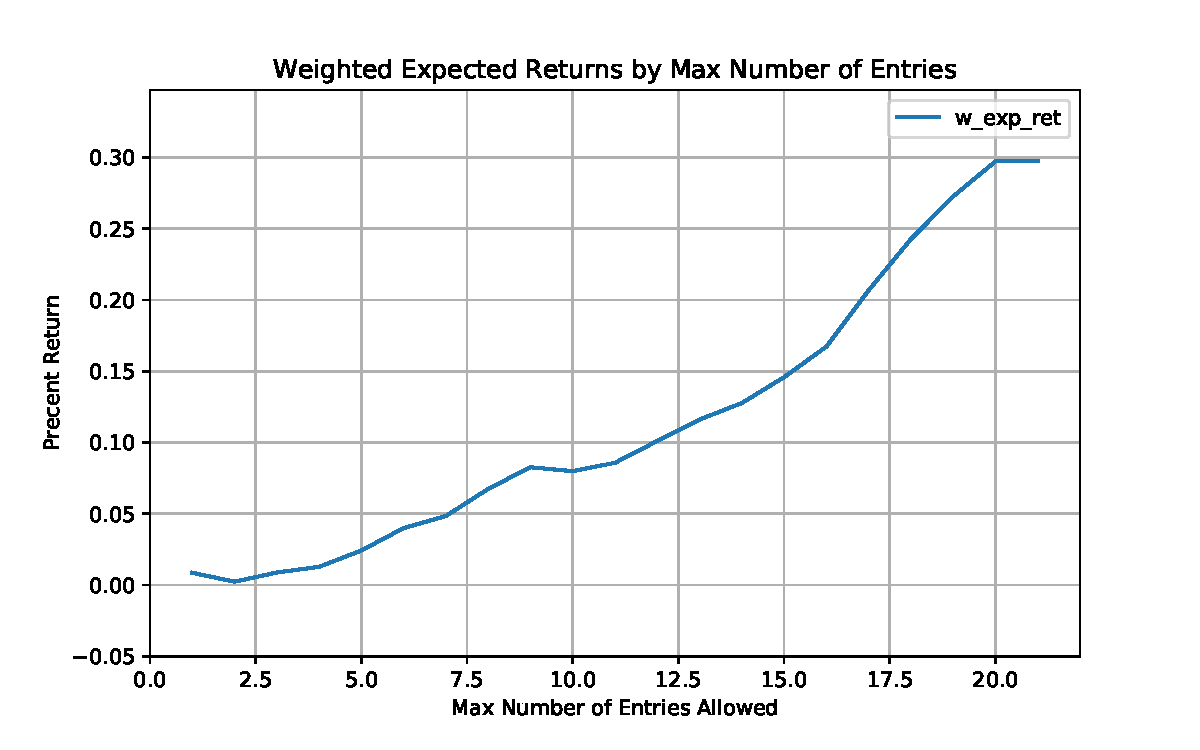
\includegraphics[width=\textwidth]{prog_entry_w_avg.pdf}
	\caption{This plot shows the weighted expected return to a limited version of the main strategy. Returns are weighted by their position size. Trades with more adds have higher weight. The returns on trades with higher weight have a larger affect on the weighted average than they would in an unweighted average. The x-axis displays the maximum number of entries allowed in a single trade. In the unlimited case, a trade can be entered each time it rises 5\%. But in the case where adds are limited to 4, the total number of entries allowed in any stock is 5 (first entry then 4 adds). So this plot says that when the maximum amount of entries is 5 (i.e. at most 4 adds) the weighted returns were around 2.5\%. When the amount of entries is limited to 5 (first entry, 4 adds), stocks that rise more than 25\% beyond the signal of 20\% are not added to beyond the first 4 adds.}
	\label{w_avg_strat}
	\end{figure}
	
	\item three plot
	
	\begin{figure}
	\center{Win Rate, Unweighted Average Return, and Average Win/Loss for  Unlimited Adds, Exit at 11 a.m.}
	
	
	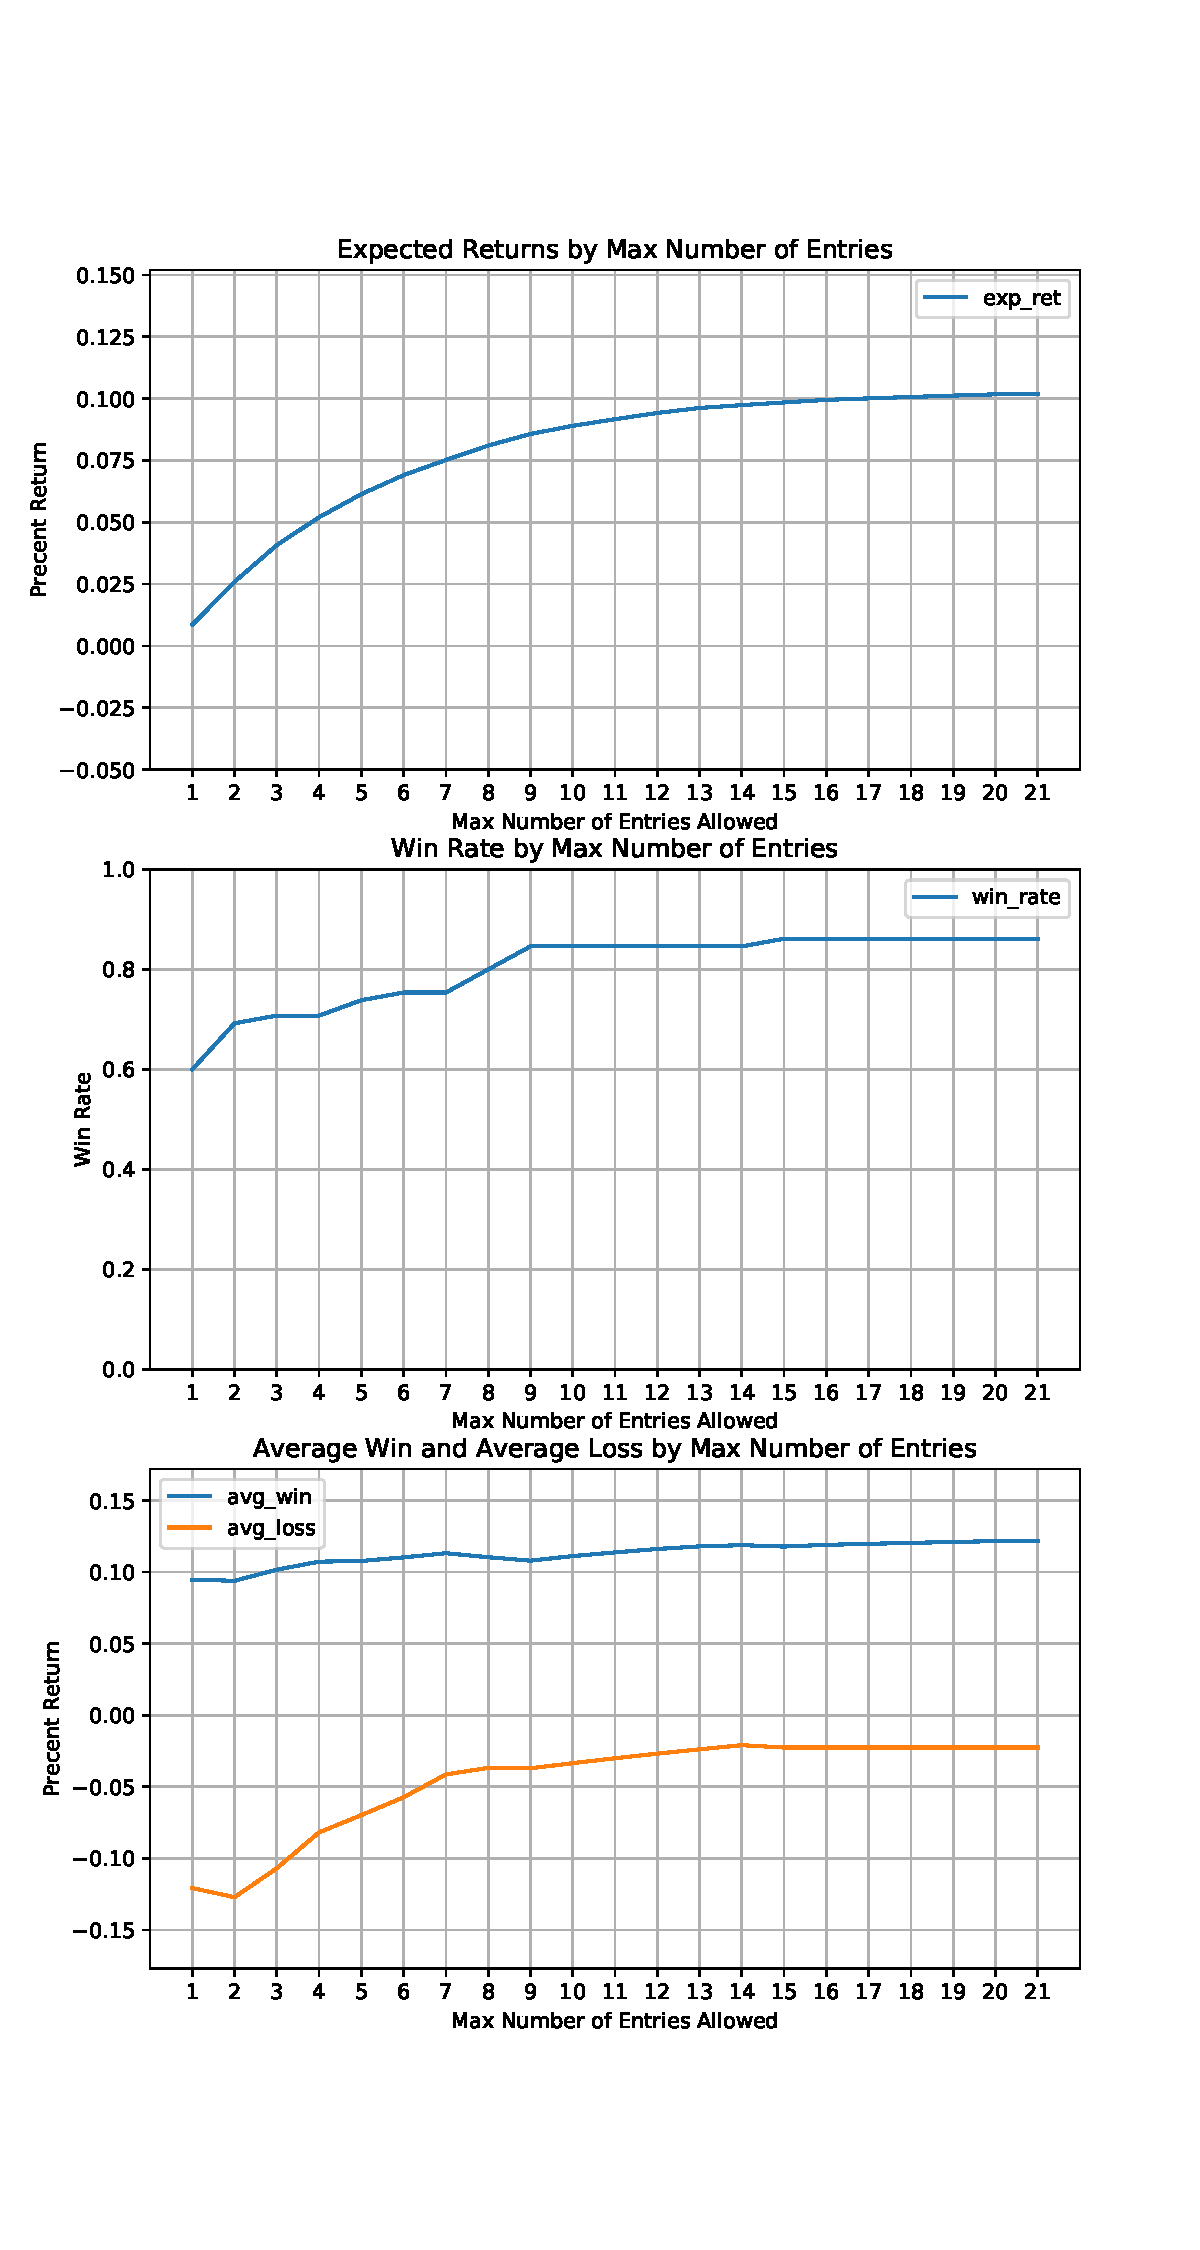
\includegraphics[width=0.6\textwidth]{prog_entry_3plot.pdf}
	\caption{The x-axis displays the maximum number of entries allowed in a single trade. In the unlimited case, a trade can be entered each time it rises 5\%. But in the case where adds are limited to 4, the total number of entries allowed in any stock is 5 (first entry then 4 adds). So the top panel says that when the maximum amount of entries is 5 (i.e. at most 4 adds) the returns were around 5.75\%. When the amount of entries is limited to 5 (first entry, 4 adds), stocks that rise more than 25\% beyond the signal of 20\% are not added to beyond the first 4 adds.}
	\label{3plot_strat}
	\end{figure}
	
	\item weighted expected return calculation: 29.7\%
\end{itemize}

\section{Alternate Strategy A: Adds Limited to 2, Exit at 11}

percent of trades with 2 or more adds, 47\%

\subsection{Analysis}

\begin{itemize}
	\item three tables
	
\begin{table}
\caption{Performance of Max 3 Adds, Exit at 11 a.m.}
\center{Overall}
\\[2ex]
\begin{tabular}{lcccc}
\hline
         &   0.1    &   0.9    &  median  & average   \\
\midrule
\midrule
constant & -0.1434  & 0.1709   & 0.0468   & 0.0408    \\
         & (0.0444) & (0.0204) & (0.0191) & (0.0160)  \\
N        & 65       & 65       & 65       & 65        \\
Win rate & 0.71     & 0.71     & 0.71     & 0.71      \\
\hline
\end{tabular}

\center{Winners}
\\[2ex]
\begin{tabular}{lcccc}
\hline
         &   0.25   &   0.75   &  median  & average   \\
\midrule
\midrule
constant & 0.0353   & 0.1593   & 0.0919   & 0.1018    \\
         & (0.0163) & (0.0220) & (0.0167) & (0.0116)  \\
N        & 46       & 46       & 46       & 46        \\
Win rate & 0.71     & 0.71     & 0.71     & 0.71      \\
\hline
\end{tabular}

\center{Losers}
\\[2ex]
\begin{tabular}{lcccc}
\hline
          &  0.25  &  0.75  &  median  & average   \\
\midrule
\midrule
constant  & 0.0307 & 0.1774 & 0.0657   & 0.1069    \\
          & (nan)  & (nan)  & (0.0391) & (0.0242)  \\
N         & 19     & 19     & 19       & 19        \\
Loss rate & 0.29   & 0.29   & 0.29     & 0.29      \\
\hline
\end{tabular}
\label{tab_strat_lim3}
\end{table}
	
	\item weighted expected return calculation: 0.9\%
\end{itemize}

\section{Alternate Strategy B: Adds limited to 2, Exit at Close}

percent of trades with 2 or more adds, 41\%

146 trades between February 26th and May 28th. 

\subsection{Analysis}

\begin{itemize}
	\item histogram
	
	\begin{figure}
	\center{Histogram of Trades by Number of Entries for Unlimited Adds, Exit at Close}
	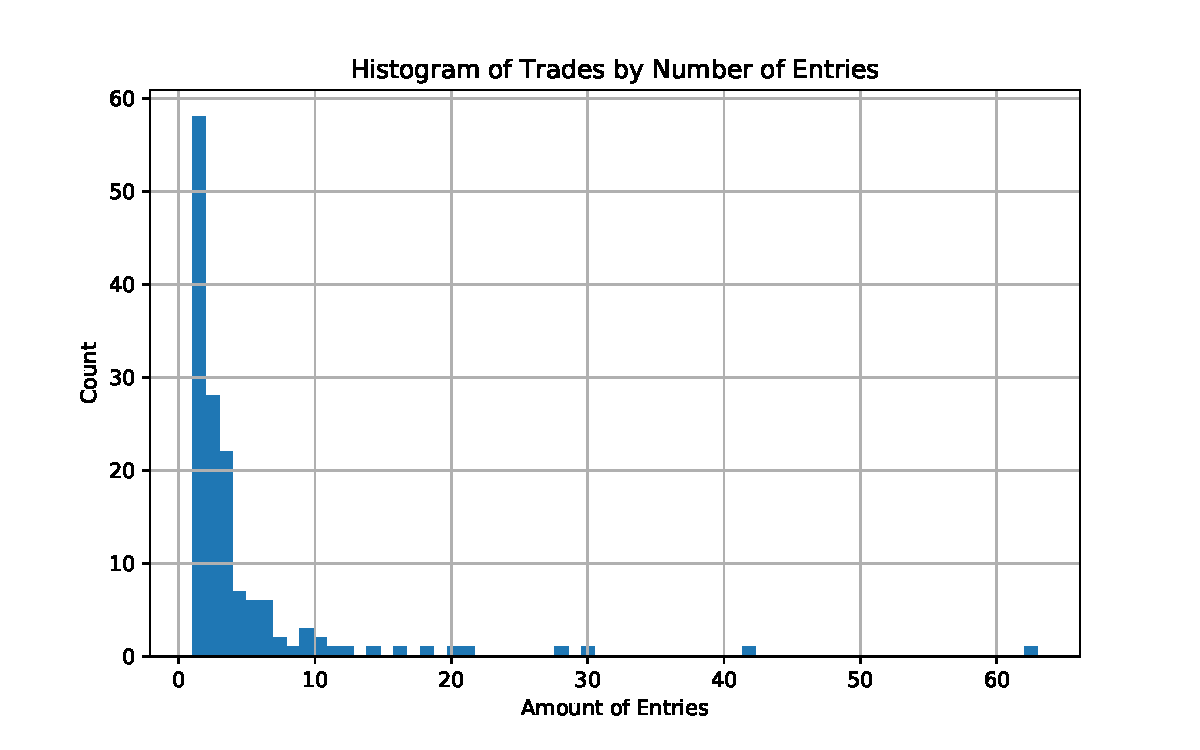
\includegraphics[width=\textwidth]{prog_entry_exit4_hist.pdf}
	\caption{This table shows counts of the numbers of trades that had a certain amount of entries. For example, it says that around 57 trades had only 1 entry, and that around 3 trades had 9 entries (fist entry and 8 adds).}
	\label{hist_strat_exit4}
	\end{figure}
	
	\item three tables
	
	\begin{table}
\caption{Performance of Max 2 Adds, Exit at Close}
\center{Overall}
\\[2ex]
\begin{tabular}{lcccc}
\hline
         &   0.1    &   0.9    &  median  & average   \\
\midrule
\midrule
constant & -0.0307  & 0.1917   & 0.1110   & 0.0969    \\
         & (0.0331) & (0.0076) & (0.0083) & (0.0085)  \\
N        & 146      & 146      & 146      & 146       \\
Win rate & 0.89     & 0.89     & 0.89     & 0.89      \\
\hline
\end{tabular}

\center{Winners}
\\[2ex]
\begin{tabular}{lcccc}
\hline
         &   0.25   &   0.75   &  median  & average   \\
\midrule
\midrule
constant & 0.0844   & 0.1610   & 0.1211   & 0.1241    \\
         & (0.0073) & (0.0070) & (0.0074) & (0.0053)  \\
N        & 130      & 130      & 130      & 130       \\
Win rate & 0.89     & 0.89     & 0.89     & 0.89      \\
\hline
\end{tabular}

\center{Losers}
\\[2ex]
\begin{tabular}{lcccc}
\hline
          &  0.25  &  0.75  &  median  & average   \\
\midrule
\midrule
constant  & 0.0516 & 0.1774 & 0.0916   & 0.1247    \\
          & (nan)  & (nan)  & (0.0455) & (0.0264)  \\
N         & 16     & 16     & 16       & 16        \\
Loss rate & 0.11   & 0.11   & 0.11     & 0.11      \\
\hline
\end{tabular}
\label{tab_strat_lim3_exit4}
\end{table}

	\item weighted expected return calculation: 7.6\%
\end{itemize}

\end{document}